\documentclass[11pt]{article}

\usepackage{float}
\usepackage{hyperref}
\usepackage{graphicx}
% formatting
\usepackage{fullpage}
\usepackage{verbatim}
\usepackage{moreverb}
\usepackage{minted}
\usepackage{parskip}
\let\verbatiminput=\verbatimtabinput
\def\verbatimtabsize{4\relax}

\begin{document}
\title{EE142 Lab 0.5 - VNA Calibration}

\author{Vighnesh Iyer \\
TAs: Vighnesh Iyer, George Alexandrov \\Department of Electrical Engineering and Computer Sciences\\
College of Engineering, University of California, Berkeley}
\date{}
\maketitle

\section{Testing Cable Phase Stability}
We connect a SMA cable between port 1 and 2. 

Before connecting the cable, the SMA connector's pin depth and dielectric depth are both checked and are within spec. Also, the SMA connector was examined under a stereo microscope and it was cleaned with a cotton swab and alcohol to remove surface contaminants (specks of dirt and metal fragments).

\begin{figure}[H]
	\minipage{0.50\textwidth}
	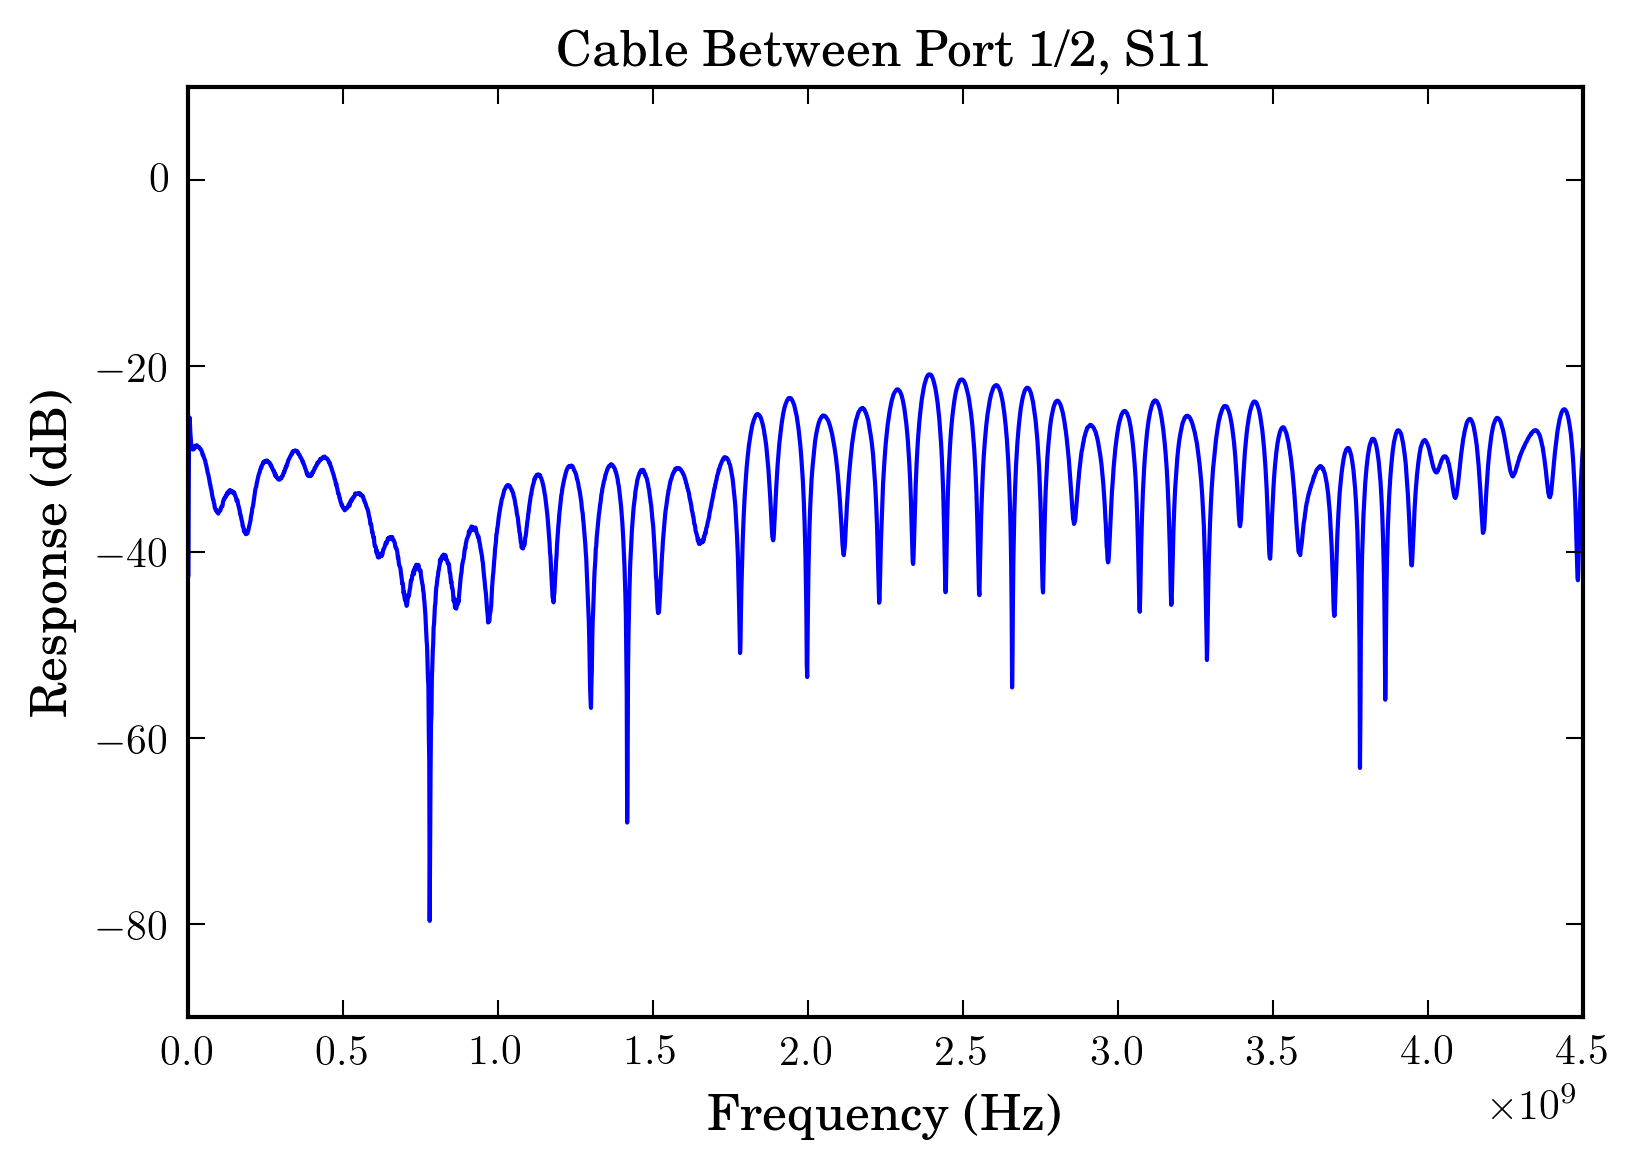
\includegraphics[width=\linewidth]{images/cable_phase_s11.png}
	\endminipage\hfill
	\minipage{0.50\textwidth}
	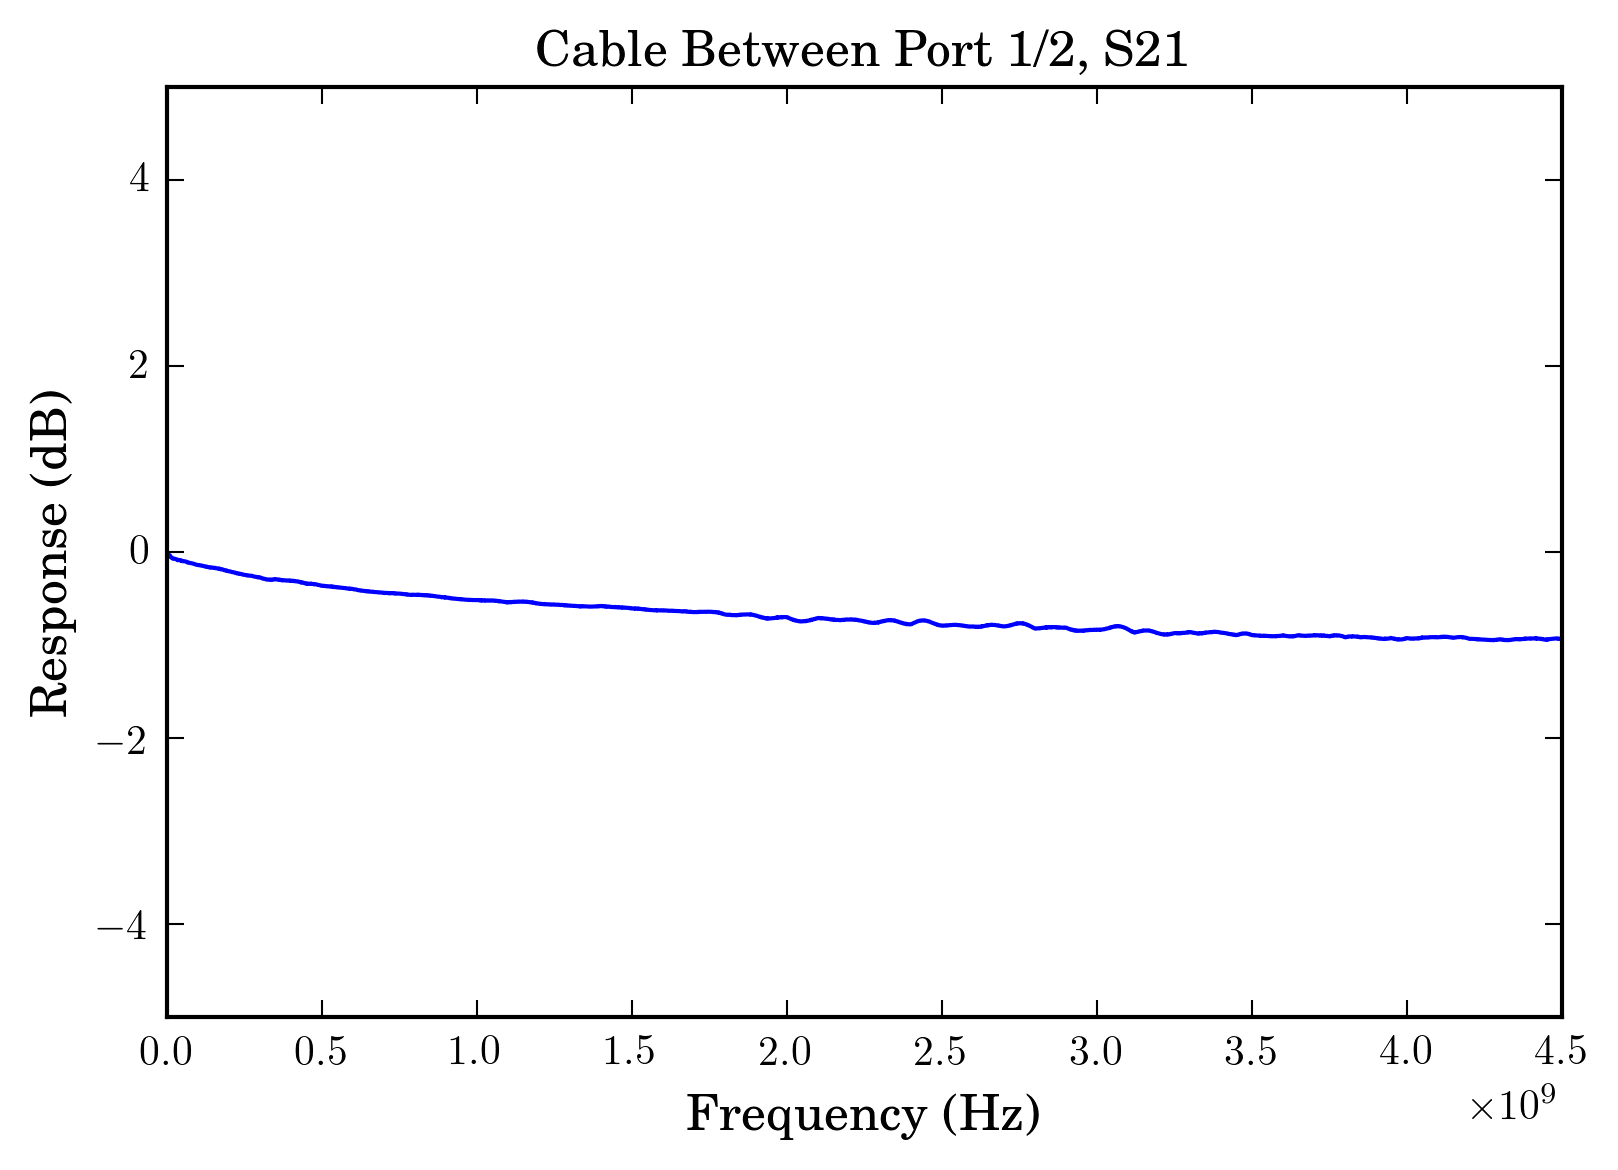
\includegraphics[width=\linewidth]{images/cable_phase_s21.png}
	\endminipage
\end{figure}

When plotting $S_{11}$, we see reflections and re-reflections 20 dB down which reflect both imperfections in the cable's impedance and possible factory calibration issues in the VNA. When measuring $S_{21}$, we see that almost all the delivered power from port 1 makes its way to port 2 and we only see some drop-off at high frequencies, where the VNA itself might be out-of-cal.

\section{}


\end{document}
